\subsubsection{VLAN de~\nameref{itm:vlan40}}
\par Para continuar con el estudio de las fuentes de paquetes ARP en distintas redes,
propusimos \textit{sniffear} una red local no tan convencional como lo son las
redes de computadoras ethernet o \textit{Wi-Fi}. Por ello trabajamos sobre una
red de telefon\'ia IP.

\par En esta redes los protocolos utilizados son los mismos que se vienen viendo
durante todo el trabajo. Aunque claramente, al ser los dispositivos tel\'efonos,
se espera ver un comportamiento distinto. En particular, este comportamiento
depender\'a de los dispositivos que componen a la red: los tel\'efonos IP.

\par Es de conocimiento en el \'area donde se ha realizado la tarea de recolecci\'on
datos, que estos dispositivos suelen tener comportamientos inesperados. De hecho,
en varios casos experimentados se observo como ciertas impresoras IP realizaban
env\'ios de paquetes \textit{broadcast} sin cesar, saturando el medio compartido
y, en la jerga informal, \textit{tirar abajo la red.}

\par Comenzamos como ven\'imos haciendo hasta ahora, con la entrop\'ia y los
datos generales de los datos obtenidos:

\begin{table}[!h]
\centering
  \begin{tabular}{c c}
    Fuente de Datos & Entrop\'ia \\
    \hline\hline
    Direcci\'on Origen & 0.0218949 \\
    Direcci\'on Destino & 5.20051 \\
    \hline\hline
    \#IPs de las Fuentes & 47\\
    \#Paquetes Capturados & 40034 \\
    \hline
    \end{tabular}
  \bigskip
  \caption{Entrop\'ia VLAN \nameref{itm:vlan40}}
  \label{tab:vlan40_entropia}
\end{table}

\par Ya de inmediato podemos ver que nos encontramos ante una LAN distinta. La entrop\'ia
de la fuente de origen es muy baja, lo cual nos da la pauta de que saber quienes son
los dispositivos que env\'ian paquetes ARP no deber\'ia ser algo incierto, sino todo
lo contrario.

\par Esto es entendible debido a que se ve que nos encontramos ante una red "peque\~na",
al menos considerando los 2 casos anteriores.


\subsubsection*{\underline{VLAN \nameref{itm:vlan40}: Fuente Origen}}\label{subsubsec:vlan40_src}
\par Veamos entonces como son las probabilidades de estas direcciones.

\begin{figure}[!ht]
    \centering
    \includegraphics[width=0.5\textwidth]{escenario_1/vlan40/vlan40_src_bars_percentile90}
    \caption{Probabilidades VLAN \nameref{itm:vlan40} - Fuente Origen}
    \label{fig:vlan40_src_prob_per90}
\end{figure}

\par Como se puede observar en la figura \ref{fig:vlan40_src_prob_per90}, ni siquiera
es necesario trabajar con el percentil 90. Hay tan pocas IPs, y -aparentemente- los
tel\'efonos no indundan la VLAN con paquetes de ARP. Esto podr\'ia deberse a muchos
distintos factores, como la configuraci\'on de estos y el software que utilizan%
\footnote{Es porbable que muchos tel\'efonos no requieran de enviar paquetes ARP ya
que por ah\'i memorizan la \textit{MAC} de la \textit{PBX} en caso de estar esta
en su LAN.}.

\par En cualquier caso, conviene observar que ocurre con la fuente de destino.
De momento lo \'unico que podemos decir es que los tel\'efonos no parecen
env\'iar demasiados paquetes ARP en la red.


\subsubsection*{\underline{VLAN \nameref{itm:vlan40}: Fuente Destino}}\label{subsubsec:vlan40_dst}

\begin{figure}[!ht]
    \centering
    \includegraphics[width=0.5\textwidth]{escenario_1/vlan40/vlan40_dst_bars_percentile90}
    \caption{Probabilidades VLAN \nameref{itm:vlan40} - Fuente Destino}
    \label{fig:vlan40_dst_prob_per90}
\end{figure}

\par Nuevamente nos encontramos con un caso impensado\footnote{Para el estudiante al menos}
en un principio. Se puede observar en la figura \ref{fig:vlan40_dst_prob_per90} que al
contrario de lo que ocurre  en la fuente de origen, en la red de telefon\'ia IP los dispositivos
tienen una distribuci\'on de la probabilidad aproximadamente equiprobable. Es decir, cada
tel\'efono, en su mayor\'ia, tiene la misma probabilidad que el resto de aparecer como
un mensaje devuelto por la fuente de informaci\'on que se est\'a estudiando.

\par Esto puede ser observado no solamente por las barras de probabilidad, sino por el
crecimiento lineal del percentil90, que no sindica que las probabilidades de cada
IP est\'an aportando aproximadamente lo mismo al percentil.

\par Es esperable ver entonces que la concentraci\'on de la probabilidad deber\'ia ser
un n\'umero que se acerque a 1 (al menos, que se acerque mucho m\'as que los casos
hasta ahora estudiados). Esto se debe a que vemos que el percentil 90 se
alcanza casi teniendo en cuenta las probabilidades de todas las IPs.

\begin{table}[!h]
\centering
  \begin{tabular}{c c c c}
    Fuente& 
    Entrop\'ia & \begin{tabular}{@{}c@{}}Concentraci\'on \\ Percentil 90\end{tabular} 
    & \begin{tabular}{@{}c@{}}Concentraci\'on \\ Percentil 80\end{tabular}\\
    \hline\hline
    Origen & 0.0218949 & 0.0021\% & 0.0021\%\\
    Destino & 5.20051 & 0.681\% & 0.553\%\\
    \hline\hline
    \end{tabular}
  \bigskip
  \caption{Concentraci\'on VLAN \nameref{itm:vlan10}}
  \label{tab:vlan40_concentracion}
\end{table}

\par Efectivamente, lo que se ven\'ia reflejando ahora tambi\'en se demuestra con los
valores del cuadro \ref{tab:vlan40_concentracion}. Vemos como la entrop\'ia de la fuente
de origen es muy baja, debido a que casi toda la probabilidad de la fuente se concentra
en una \'unica direcci\'on IP (ver figura \ref{fig:vlan40_src_prob_per90}), teniendo
al mismo tiempo una concentraci\'on muy baja del percentil 90 (al fin y al cabo, es
s\'olo una IP la que acumula todo).

\par Por el otro lado, vemos que como fuente de destino, nos encontramos con una concentraci\'on
del percentil m\'as alta que en casos anteriores. El hecho de que la probabilidad
sea casi equiprobable entre todos los s\'imbolos de la fuente nos da una entrop\'ia
relativamente alta para la cantidad de IPs que se tienen en la fuente (47). Esto se
debe a que al ser equiprobable\footnote{Apr\'oximadamente} el espacio de s\'imbolos
de la fuente, hay una gran incertidumbre que no nos permite asegurar con una buena
base estad\'istica sobre quienes son los datos m\'as probables que nos dar\'a la
fuente.

\subsubsection*{\underline{VLAN \nameref{itm:vlan40}: Ambas Fuentes}}\label{subsubsec:vlan40_src_dst}
\par Dado que estamos en una red chica y, aparentemente poco densa, sumado a la
probabilidad concentrada de la fuente de origen y la distribu\'ida de la fuente destino,
nos da a entender que nos encontraremos con una topolog\'ia donde todos se comunican
con la IP \textit{5.0.48.1}\footnote{\nameref{fig:vlan40_src_prob_per90}.}.

\begin{figure}[ht]
    \centering
    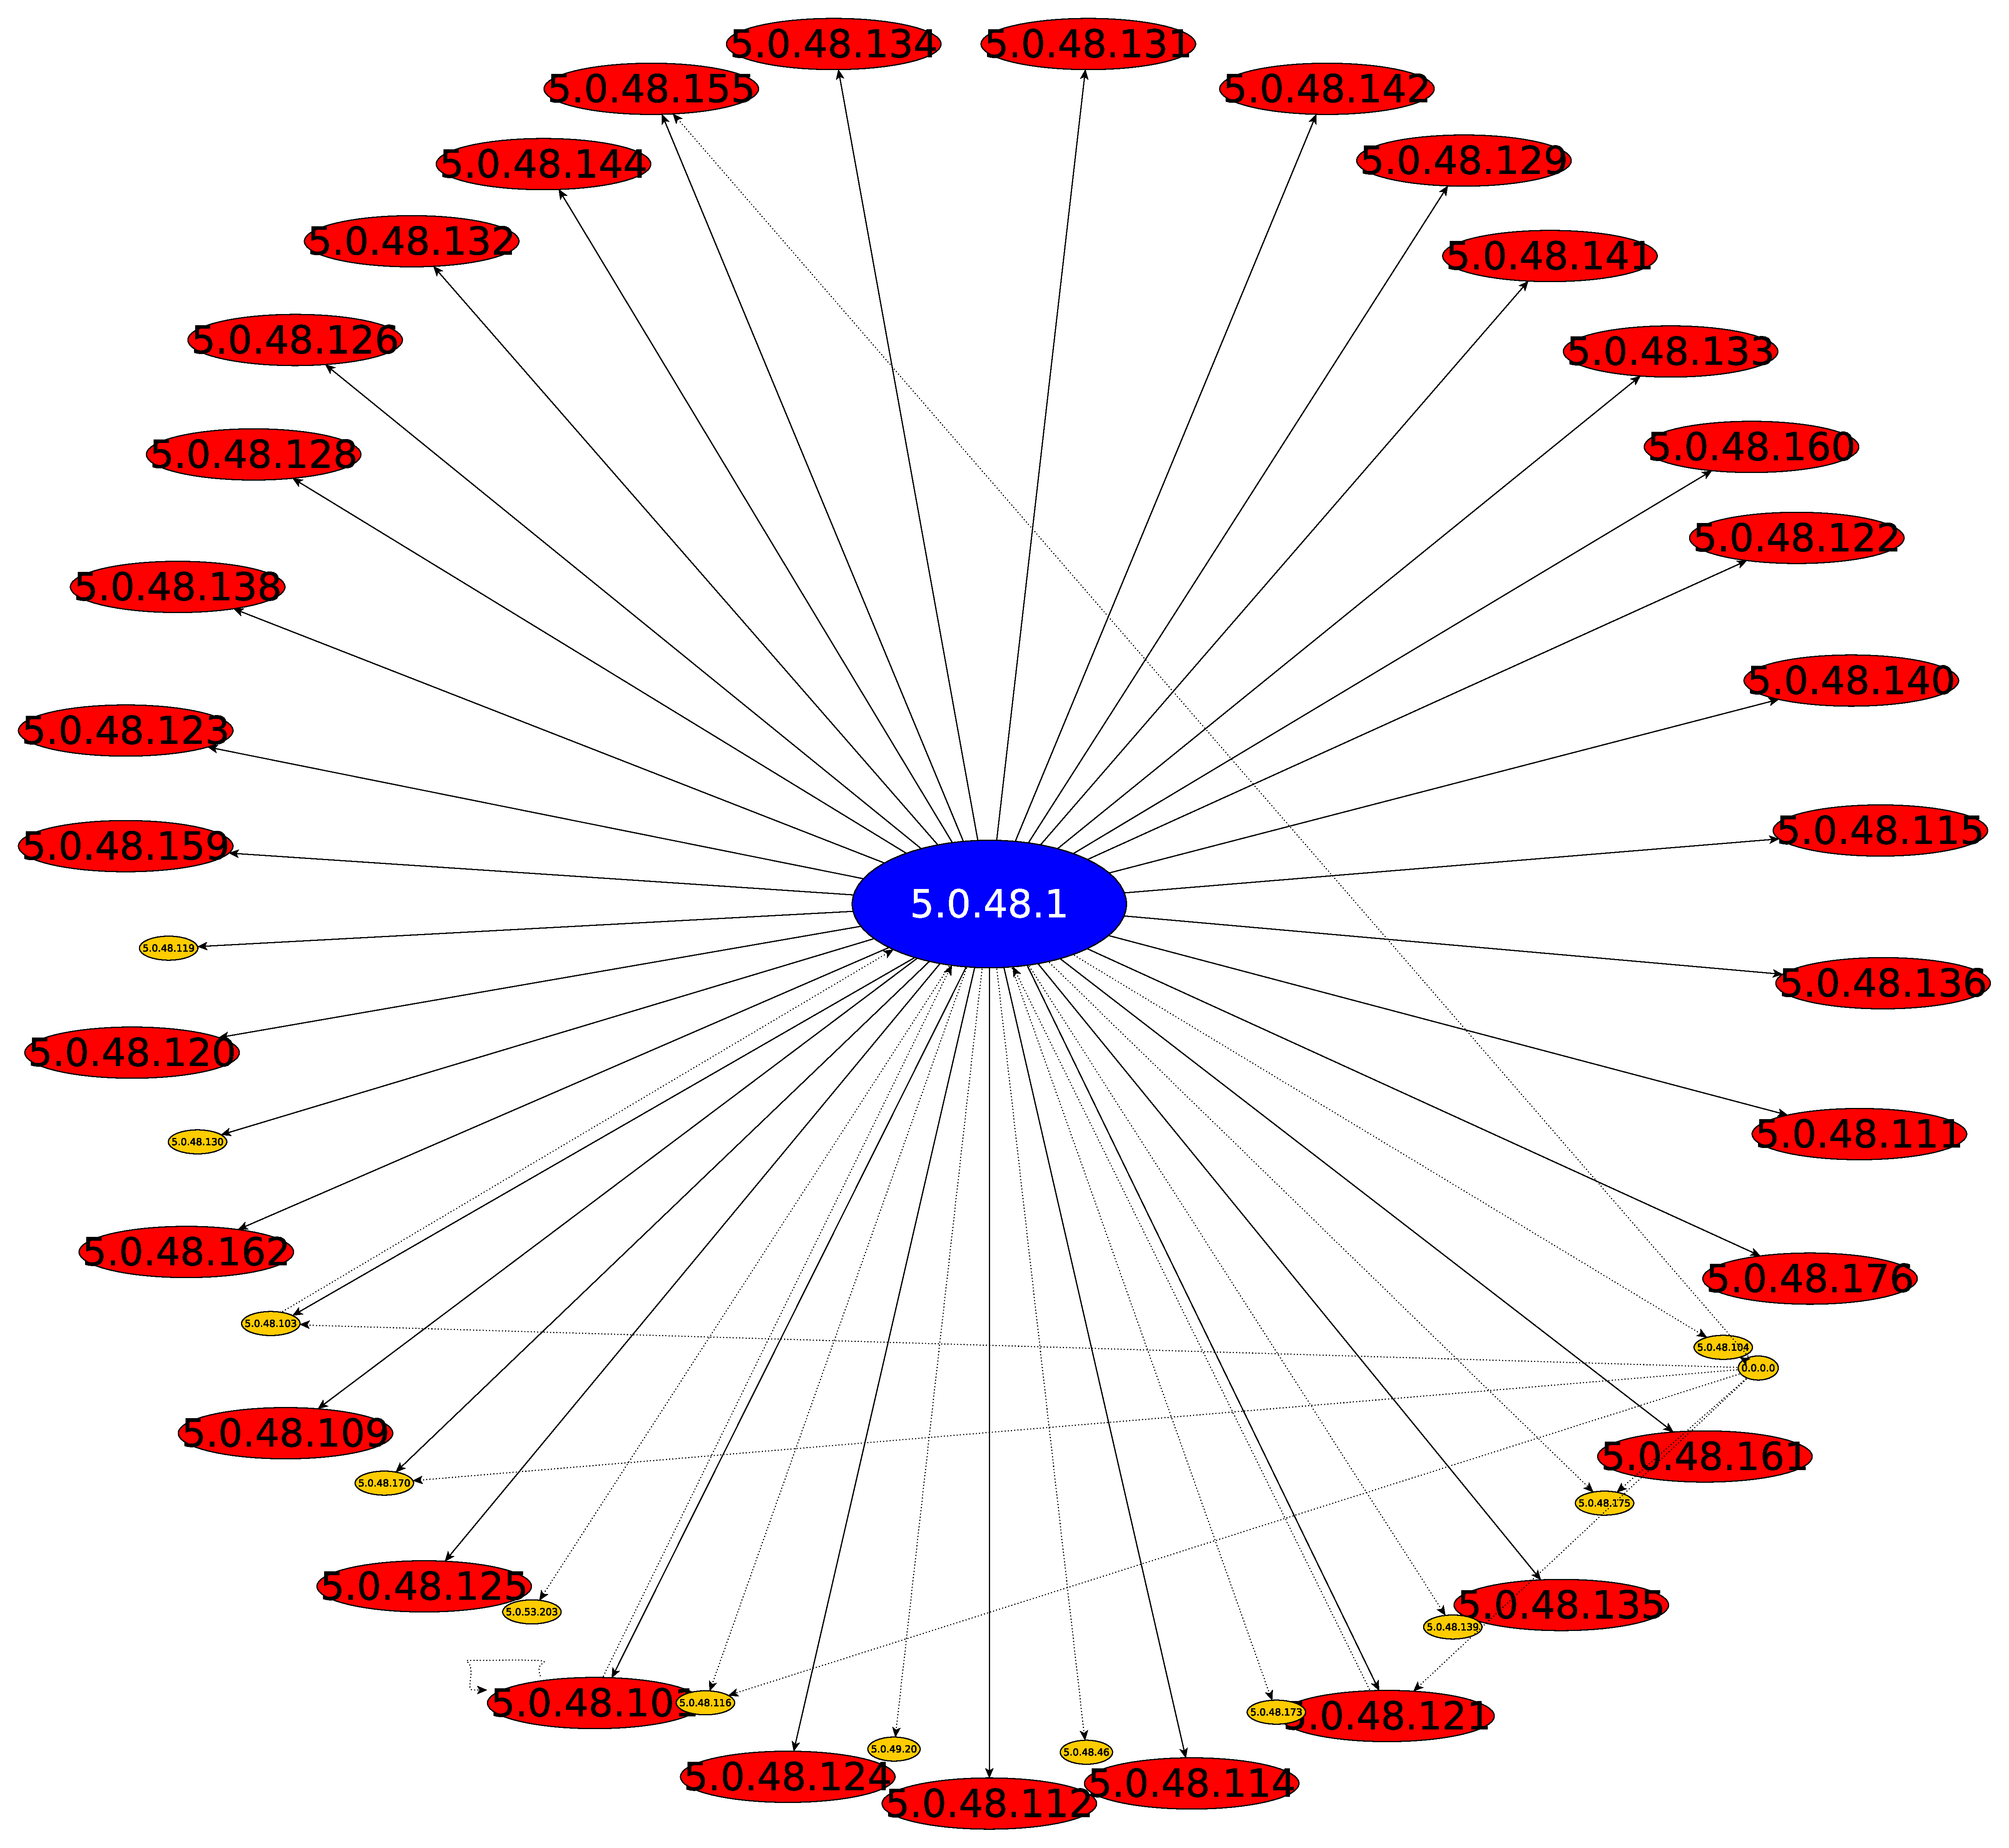
\includegraphics[width=0.5\textwidth]{img/graph/escenario_1/vlan40/vlan40}
    \caption{Grafo VLAN \nameref{itm:vlan40}}
    \label{fig:vlan40_grafo}
\end{figure}

\par Efectivamente se puede observar en el grafo que la red de tel\'efonia
IP parece trabajar con una topolog\'ia centralizada, al menos para cada vez
que deben resolver una \textit{MAC}, presumiblemente para realizar alguna
tarea que requiera de la utilizaci\'on de la red\footnote{Eso o la
telefon\'ia IP se utiliza muy poco en el datacenter.}.

\par As\'i pues, queda claro en la figura \ref{fig:vlan40_grafo} que nos encontramos
con un nodo principal que seguramente es la \textit{PBX} o servidor del
servicio de tel\'efon\'ia m\'ovil.


\subsubsection*{\underline{VLAN \nameref{itm:vlan40}: Conclusiones}}\label{subsubsec:vlan40_conclusiones}
\par Aqu\'i nos encontramos con una red que claramente se comporta distinta que el resto.
De la informaci\'on recolectada y los an\'alisis realizados, se pudo ver que
hay muy poco tr\'afico y por ende los valores de entrop\'ia y la cantidad
de IPs de la LAN nos permiten anticipar el comportamiento de la LAN sin
conocer detalles t\'ecnicos sobre la infraestructura o el software que 
utilizan los tel\'efonos.
